\documentclass[7pt]{article}

\usepackage{amsmath}
\usepackage{graphicx}
\usepackage{caption}
\usepackage[landscape]{geometry}
\usepackage{multicol}
\usepackage{amssymb}

\usepackage{geometry}
\geometry{
 a4paper,
 total={285mm,185mm},
 left=10mm,
 top=10mm,
}

\setcounter{section}{3}
\setlength\columnseprule{0.5pt}
\setlength{\parindent}{0pt}
\graphicspath{ {images/} }

\begin{document}
\begin{multicols*}{3}

\section{Energie}

\subsection{Energieerhaltung}

Bei allen Vorg{\"a}ngen muss die Gesamtenergie eines Systems und seiner Umgebung erhalten werden.
\begin{equation*}
	E_{tot} = E_{Masse} + E_{kin} + E_{pot} + E_{chem} + \text{usw.} = \text{konst.}
\end{equation*}

\subsection{Relativistische Gr{\"o}ssen}

\begin{equation*}
	\text{Geschwindigkeitsparameter} \equiv \frac{v}{c}
\end{equation*}

F{\"u}r hohe Geschwindigkeiten giltet der relativistische Impuls:
\begin{equation*}
	p = \gamma mv
\end{equation*}

mit dem \textbf{Lorentzfaktor $\gamma$}
\begin{equation*}
	\gamma \equiv \frac{1}{\sqrt{1-\frac{v^2}{c^2}}}
\end{equation*}

\subsection{Kinetische Energie}

\subsubsection{Klassisch ($v < 0.3c$)}

\textbf{Gesamtenergie}
\begin{equation*}
	E = mc^2 + \frac{1}{2}mv^2
\end{equation*}

\textbf{Kinetische Energie}
\begin{equation*}
	E = \frac{1}{2}mv^2
\end{equation*}

\subsubsection{Relativistisch ($v \geq 0.3c$)}

\textbf{Gesamtenergie}
\begin{equation*}
	E = \gamma mc^2 = \frac{mc^2}{\sqrt{1-\frac{v^2}{c^2}}}
\end{equation*}
\begin{equation}
	E=\sqrt{c^2p^2+m^2c^4}
\end{equation}

\textbf{Kinetische Energie}
\begin{equation*}
	E_{kin} = E - mc^2 = mc^2(\gamma - 1)
\end{equation*}

\subsection{Potentielle Energie der Gravitation}

Die \textbf{potentielle Energie} eines K{\"o}rpers auf der H{\"o}he $h$ ist gleich
\begin{equation*}
	E_{pot}(h) = mgh
\end{equation*}

Die \textbf{Gesamtenergie} eines K{\"o}rpers im freien Fall von der H{\"o}he $h$ ist gleich
\begin{equation*}
	E(y) = \underbrace{mc^2}_\text{Ruheenergie} + \underbrace{\frac{1}{2}mv^2}_\text{kinetisch} + \underbrace{mgy}_\text{potentiell}
\end{equation*}

falls der \emph{Luftwiderstand} vernachl{\"a}ssigt werden darf.

\subsection{Looping}

\begin{center}
	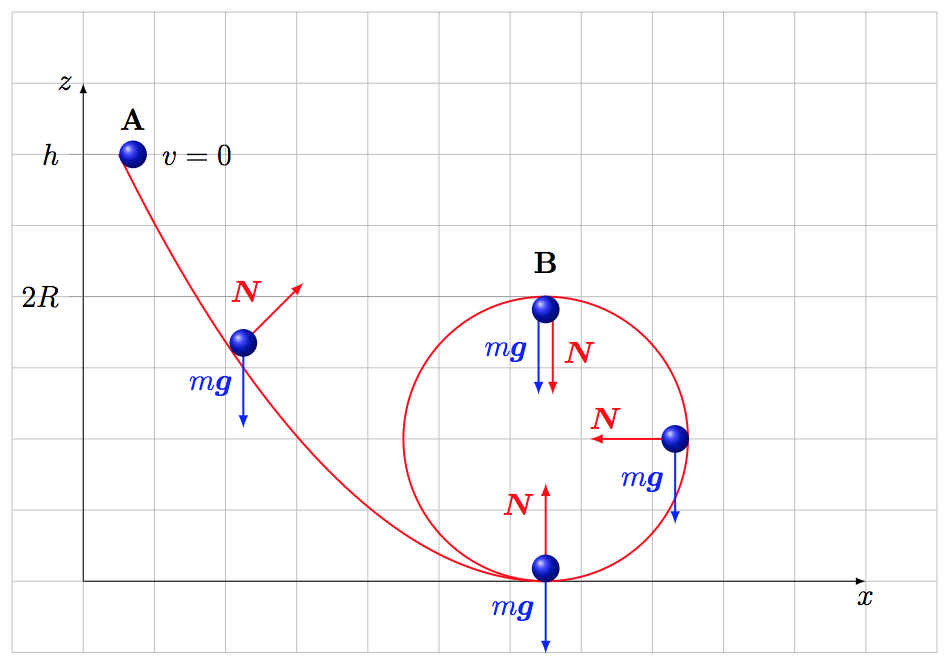
\includegraphics[width=200pt]{images/looping}
\end{center}

Ist die Geschwindigkeit kleiner als $v_{min}$, l{\"o}st sich der Ball vom Kreis
\begin{equation*}
	v_{min} = \sqrt{gR}
\end{equation*}

Die H{\"o}he $h$, von der die Kugel fallen gelassen werden muss, ist gleich
\begin{equation*}
	h = \frac{5}{2}R > 2R
\end{equation*}

\subsection{Arbeit}

Die \textbf{Arbeit $W$} ist gleich dem Produkt der Komponente der Kraft \underline{l{\"a}ngs der Verschiebung} und der Verschiebung selbst
\begin{equation*}
	W = F\Delta x\cos(\vartheta)
\end{equation*}

\subsubsection{Arbeit der Federkraft}

Die \textbf{Arbeit} zwischen den Verschiebungen $x_1$ und $x_2$ ist gleich
\begin{equation*}
	W_{12} = -\frac{k}{2}(x_2^2-x_1^2)
\end{equation*}

\subsection{Leistung}

Die \textbf{Leistung $P$} ist die in der Zeiteinheit verrichtete Arbeit:
\begin{equation*}
	P = \frac{dW}{dt} = F \cdot v
\end{equation*}

\subsection{Allgemeine potentielle Energie}

\subsubsection{Konservative Kr{\"a}fte}
Die geleistete Arbeit l{\"a}ngs eines geschlossenen Wegs ist gleich null. Die Arbeit ist unabh{\"a}ngig vom zur{\"u}ckgelegten Weg.\underline{Potentielle Energie ist f{\"u}r diese Art von Kr{\"a}ften definiert.}\newline
\emph{Beispiel:} Gravitationskraft, Federkraft

\subsubsection{Nicht-konservative Kr{\"a}fte}
Die geleistete Arbeit h{\"a}ngt vom Weg ab. \newline
\emph{Beispiel:} Reibungskraft

\subsection{Arbeit-Energie-Theorem}

Die Arbeit, die an einem K{\"o}rper zwischen zwei Punkten (1) und (2) geleistet wird, ist gleich der {\"a}nderung seiner kinetischen Energie zwischen diesen Punkten.
\begin{equation*}
	W_{12} = \frac{1}{2}mv_2^2 - \frac{1}{2}mv_1^2
\end{equation*}

\subsection{Mechanische Energie}

\begin{equation*}
	E_{mech} \equiv E_{kin} + E_{pot}
\end{equation*}

Die mechanische Energie wird \emph{erhalten}, wenn nur konservative Kr{\"a}fte wirken. \newline
Die {\"a}nderung der mechanischen Energie ist gleich der Arbeit, die von \emph{nicht-konservativen} Kr{\"a}ften geleistet wird.

\subsection{Bremsweg}

Betrachtet wird das Gleiten auf einer \textbf{schiefen} Ebene mit der Starth{\"o}he $h$ und dem Neigungswinkel $\vartheta$. Dann ist der \textbf{Bremsweg $L$}

\begin{equation*}
	L = \frac{v_0^2}{2g(\mu\cos(\vartheta) - \sin(\vartheta)}
\end{equation*}

Ist die Ebene \textbf{waagrecht}, so gilt:

\begin{equation*}
	L = \frac{v_0^2}{2a}
\end{equation*}

\end{multicols*}
\end{document}